%\begin{figure}[h]
%    \centering
%	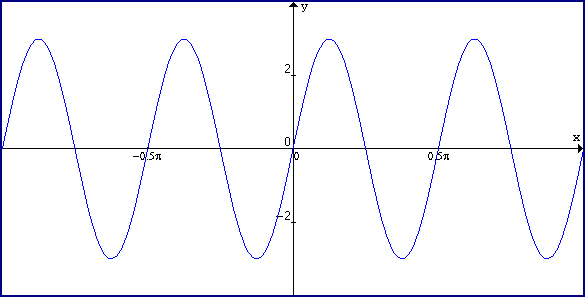
\includegraphics[scale=0.5]{graph}
%	\caption{An example graph}
%	\label{fig:x sine graph}
%\end{figure}


\newcommand{\featcount}{V}
\newcommand{\traj}{y}
\newcommand{\embed}{\vect{v}}
\newcommand{\df}{DF}
\newcommand{\featset}{\text{M}}
\newcommand{\cost}{\text{C}}

\newcommand{\semsim}{\text{Sim}}
\newcommand{\featsim}{\text{JSD}}

\newcommand{\bowmat}{\mat{B}}
\newcommand{\dtdmat}{\mat{D}}
\newcommand{\trajmat}{\mat{T}}


The goal of this phase is to discover sets of word features highly correlated both semantically and in the time domain. The assumption is that if a group of words suddenly appears with higher frequency in a given time window and has similar meaning, it concerns the same real world event. If we extract a sample of meaningful words out of those, they can be used to concisely represent an event. Using these words, we can query the document collection to obtain document representation of the events as well.

The core of this algorithm is taken from \cite{event-detection}.


\section{Binary bag of words model}
Apart from word embeddings, we will use yet another vector representation of the word features. This time, the vectors will represent trajectories of word frequency in time. Each word feature $f$ will in the end be represented by two vectors; $\vect{\traj}_{f}$ being its time trajectory, and $\embed_{f}$ being its semantic word embedding.

We first adapt the binary form of the standard bag of words model to obtain a term-document matrix $\bowmat \in \left\{ 0, 1 \right\}^{\doccount \times \featcount}$, where $\featcount$ is the total vocabulary size. The document collection can then be interpreted as a set of $\doccount$ observations, each consisting of $\featcount$ binary features. The matrix $\bowmat$ is defined as

\begin{equation} \label{eq:bow-matrix}
	\bowmat_{ij} \coloneqq
	\begin{cases}
		1, & \text{document}~i~\text{contains the feature}~j \text{;} \\
		0, & \text{otherwise.}
	\end{cases}
\end{equation}

{\color{red} TODO: Figure out the min\_freq and max\_freq of words to keep.}

To limit the feature space, we trim the words appearing in less than 30 documents or in more than 90\% of the documents. The idea behind this is that the words appearing only in few documents cannot possibly represent relevant events, and are mostly anomalies. On the other hand, words appearing in most of the documents are likely stopwords, and do not carry much information. This helps to prune the feature space and makes $\bowmat$ reasonably sized.

From now on, we focus our analysis on the individual word features rather than whole documents.


\section{Computing feature trajectories}
The time trajectory of a feature $f$ is a vector $\vect{\traj}_f = \left[ \traj_{f}(1), \traj_{f}(2), \dots, \traj_{f}(\streamlen) \right]$ with each element $\traj_{f}(t)$ representing the relative frequency of $f$ at time $t$. This frequency is defined using the DFIDF score:

\begin{equation}
	\traj_{f}(t) \coloneqq \underbrace{\frac{\text{\df}_{f}(t)}{\text{\doccount}(t)}}_{\text{DF}} \cdot \underbrace{\log{\frac{\doccount}{\text{\df}_{f}}}}_{\text{IDF}},
\end{equation}

where $\text{\df}_{f}(t)$ is the number of documents published on day $t$ containing the feature $f$ (time-local document frequency), $\text{\doccount}(t)$ is the number of documents published on day $t$ and $\text{\df}_{f}$ is the number of documents containing the feature $f$ (global document frequency).

These feature trajectories are stored in a matrix $\trajmat \in \R^{\featcount \times \streamlen}$, with $\vect{\traj}_f$ being the $f$-th row of $\trajmat$. Here we take advantage of the normalization of the publication days, since they can now be used as column indices of $\trajmat$.

To make the computation efficient, we vectorize most of the operations. Along with the matrix $\bowmat$ defined in \ref{eq:bow-matrix}, we define a matrix $\dtdmat \in \left\{ 0, 1 \right\}^{\doccount \times \streamlen}$ mapping the documents to their publication days:

\begin{equation}
	\dtdmat_{ij} \coloneqq
	\begin{cases}
		1, & \text{document}~i~\text{was published on day}~j \text{;} \\
		0, & \text{otherwise}.
	\end{cases}
\end{equation}

Next, we sum the rows of $\bowmat$ together to obtain $\vect{\df} = \left[ \text{\df}_{1}, \text{\df}_{2}, \dots, \text{\df}_{\featcount} \right]$, and similarly the rows of $\dtdmat$ to obtain $\vect{\doccount}_{t} = \left[ \text{\doccount}(1), \text{\doccount}(2), \dots, \text{\doccount}(\streamlen) \right]$.

Using these matrices and vectors, we can compute $\trajmat$ as follows:

\begin{equation}
	\trajmat \coloneqq
		\underbrace{\text{diag} \left( \log{\frac{\doccount}{\vect{\df}}} \right)}_{\text{IDF}}
		\cdot
		\underbrace{\bowmat^{\T}
		\cdot \dtdmat
		\cdot \text{diag} \left( \frac{1}{\vect{\doccount}_{t}} \right)}_{\text{DF}}
\end{equation}


\section{Spectral analysis}
In this section, we interpret each feature trajectory as a time signal, which allows us to employ spectral analysis techniques to discover periodicities and estimate signal power of the features. Results from this section are then used to extract only a fraction of features with high overall frequency and to distinguish between periodic and aperiodic features.

We apply the discrete Fourier transform to each feature trajectory, which represents the time series as a linear combination of $\streamlen$ complex sinusoids. We obtain $\mathcal{F} \vect{\traj}_{f} = \left[ X_{1}, X_{2}, \dots, X_{\streamlen}\right ]$ such that

\begin{equation*}
	X_{k} = \sum_{t = 1}^{\streamlen}{\traj_{f}(t) \exp(- \frac{2 \pi \mi}{\streamlen} (k - 1) t}), ~ k = 1, 2, \dots, \streamlen.
\end{equation*}

The absolute value of the Fourier coefficient $X_{k}$ denotes the amplitude of the complex sinusoid at frequency $\frac{k}{\streamlen}$.

Having moved from the time domain to the frequency domain, we can now analyze the signal power and dominant periodicity of each feature.

We observe peaks in the power spectrum of the transformed data and obtain the signal power and periodicity from those. The power spectrum is estimated using the periodogram estimator

\begin{equation*}
	\vect{P} = \left[ \|X_{1}\|^{2}, \|X_{2}\|^{2}, \dots, \|X_{\ceil{\streamlen / 2}}\|^{2} \right].
\end{equation*}

To measure the overall signal power, we define the dominant power spectrum of the feature $f$ as the value of the highest peak in the power spectrum, that is

\begin{equation}
	\text{DPS}_{f} \coloneqq \max\limits_{k \leq \ceil{\streamlen / 2}}{\|X_{k}\|^{2}}.
\end{equation}

The dominant period is then defined as the inverse of the frequency corresponding to the highest peak:

\begin{equation}
	\text{DP}_{f} \coloneqq \frac{\streamlen}{\argmax\limits_{k \leq \ceil{\streamlen / 2}}{\|X_{k}\|^{2}}},
\end{equation}

When applied to rows of the matrix $\trajmat$, this method yields two vectors $\vect{DPS},\ \vect{DP} \in \R^{\featcount}$, containing the dominant power spectra and dominant periods, respectively.


\section{Feature categorization}
Based on the dominant power spectra and dominant periods, we divide the features into \underline{H}igh power-\underline{H}igh period and \underline{H}igh power-\underline{L}ow period categories \footnote{\cite{event-detection} actually define \textit{five} such categories; however, our method uses only the two sets of the most powerful features.}:

\begin{equation}
\begin{split}
	\text{HH} \coloneqq \left\{ f \mid \text{DPS}_{f} > \textit{dps-bound}, \text{DP}_{f} > \ceil{\streamlen / 2} \right\}, \\
	\text{HL} \coloneqq \left\{ f \mid \text{DPS}_{f} > \textit{dps-bound}, \text{DP}_{f} \leq \ceil{\streamlen / 2} \right\}.
\end{split}
\end{equation}

{\color{red}TODO: Define dps-bound!}


\section{Event detection}
To cluster the word features in both time and semantic domains, we will need to measure their distance. We first define a pairwise distance measure in each domain. These measures are then generalized to measure the distance of a feature from a whole set of features, so we can assign the closest feature to a partially constructed event. In the last step, these distances are combined into a single cost function which we aim to minimize.


\subsection{Measuring trajectory distance}

Distance between two feature trajectories is defined in terms of their information divergence. Unlike \cite{event-detection}, we use the \textit{Jensen-Shannon} divergence:

\begin{equation*}
	\featsim( \vect{p} \| \vect{q} ) = \frac{1}{2} \text{D}( \vect{p} \| \vect{m} ) + \frac{1}{2} \text{D}( \vect{q} \| \vect{m} ),
\end{equation*}

where $\vect{m} = \frac{1}{2} \left( \vect{p} + \vect{q} \right)$ and $\text{D}( \cdot \| \cdot )$ denotes the \textit{Kullback-Leibler} divergence.

Next, this measure is generalized to measure the distance between a feature set $\featset$ and another feature $f$ as

\begin{equation}
	\featsim( \featset, f ) = \featsim( \vect{\bar{\traj}}_{\featset} \| \vect{\traj}_{f} ),
\end{equation}

where $\vect{\bar{\traj}}_{\featset}$ is the mean of all trajectories of features in $\featset$ and $\vect{\traj}_{f}$ is the trajectory of feature f.

{\color{red} TODO: Move the pairwise similarities to the cluster-based algorithm, keep only the set-feature ones here.}

{\color{blue} TODO: Try KL(mean(M),f) instead of JSD(mean(M),f)? Like M is the true distribution and f assumed. Keep JSD in pairwise similarity though, clustering likes symmetry.}


\subsection{Measuring semantic similarity}

The semantic similarity is again first defined for two features, and then generalized to a similarity between a feature set and another feature. Here, we utilize the word embeddings computed in \ref{word-embeddings}.

Most of the astounding results of the word2vec model come from semantic relations between words being preserved under vector arithmetic, with words concerning the same topic having roughly the same angle. Thus, we use the cosine similarity between embeddings $\embed_{i}$ and $\embed_{j}$ of word features $i$ and $j$:

\begin{equation}
	\semsim( f_{i}, f_{j} ) \coloneqq \frac{\inp[\big]{\embed_{i}}{\embed_{j}}}{\| \embed_{i} \| \cdot \| \embed_{j} \|}
\end{equation}

Next, we generalize the similarity for a feature set $\featset$ and another feature $f$ as

\begin{equation}
	\semsim( \featset, f ) \coloneqq \semsim( \bar{\embed}_{\featset}, \embed_{f} ),
\end{equation}

where $\bar{\embed}_{\featset}$ is the mean of all vector embeddings of features in $\featset$ and $\embed_{f}$ is the vector embedding of the feature $f$. Here, the mean vector is supposed to represent a shared topic among words from $\featset$.


\subsection{Event detection}

We can now measure the similarity both in the time domain and in the semantic domain. These two measures are now combined into a single cost function $\cost$, which the algorithm will try to minimize:

\begin{equation} \label{eq:cost-function}
	\cost( \featset, f ) \coloneqq \frac{\featsim( \featset, f )}{\exp(\semsim( \featset, f )) \cdot \sum_{g \in \featset \cup f}{\text{DPS}_{g}}}
\end{equation}

We exponentiate the cosine similarity so that the resulting value is always positive. Intuitively, a set $\featset \cup f$ which minimizes this function will have low inter-trajectory divergence, high semantic coherence and will be comprised of relevant features with high DPS.

To perform the event detection itself, we mostly adapt the \textit{Unsupervised greedy event detection} algorithm from \cite{event-detection}.

\begin{algorithm}[H]
\begin{algorithmic}[1]
\caption{Unsupervised greedy event detection}
\Input $\text{Feature set} ~ F = \text{HH or HL}$

\State $\text{Sort the features in ascending DPS order: } DPS_{f_{1}} \leq \dots \leq DPS_{f_{\left\vert F \right\vert}}$

\State $k = 0$

\ForEach{$f \in F$}
	\State $k = k + 1$	
	\State $e_{k} = \{ f \}$
	\State $cost_{e_{k}} = \frac{1}{DPS_{f}}$
	\State $F = F \setminus f$
	
	\While{$F \neq \emptyset$}
		\State $m = \argmin\limits_{m}{\cost( e_{k}, f_{m} )}$

		\If{$\cost( e_{k}, f_{m} ) < cost_{e_{k}}$}
			\State $cost_{e_{k}} = \cost( e_{k}, f_{m} )$
			\State $e_{k} = e_{k} \cup f_{m}$
			\State $F = F \setminus f_{m}$
		\Else
			\Break
		\EndIf
	\EndWhile
\EndFor

\Output $\text{Events} ~ \{ e_{1}, e_{2}, \dots, e_{k} \}$
\end{algorithmic}
\end{algorithm}

We do make a change and sort the features in \textit{ascending} rather than descending order. This ensures that words with lower DPS value will get selected first and that the function \ref{eq:cost-function} will not be minimized as quickly. As a result, the events will contain more representative features and will not be broken into several parts. This effectively relaxes the DPS part of the function \ref{eq:cost-function} while keeping emphasis on the trajectory similarity and document overlap.